\chapter{\label{cnn} Machine learning for continuous wave searches}
%%%%%%%%%%
%%%%%%%%%%

%--------------------------
% Introduce machine learning
%----------------------------

Machine learning is a term which was used by Arthur Samuel in 1959. 
He described it as a "Field of study that gives computers the ability to learn without being explicitly programmed" \citep{}.
This can be though of as a subset of artificial intelligence. 

With the development in computing in recent years, including GPUs and the languages used to program with them, machine learning has become more accessible. 


%%%%%%%%%%%%
%%%%%%%%%%%%%%%
\section{\label{machine:intro} Introduction}
%%%%%%%%%%%%
%%%%%%%%%%%%%

% Intro to GWs and CW
%
Gravitational wave detectors such as \ac{LIGO}~\cite{abbott2009LIGOLaser,aasi2015AdvancedLIGO} and VIRGO
\cite{acernese2015AdvancedVirgo,acernese2008StatusVirgo} search for a number of different targets. 
Some targets such as \acp{CBC} have been observed ~\cite{abbott2017GW170817Observation,abbott2017GW170814ThreeDetector,abbott2016ObservationGravitational},
however, other primary sources such as \acp{CW} are yet to be observed.
\acp{CW} are well modelled quasi-sinusoidal signals with a
duration much longer than observing times of detectors.
The source of these signals is thought to be rapidly rotating neutron stars which can emit \ac{GW} if there is some asymmetry around its rotation axis. 
This can be caused by various mechanisms as described in ~\cite{prix2009GravitationalWaves}. 
These signals have small amplitude, which if detected will be below the noise \ac{PSD} of the detector.
Therefore, sensitive search algorithms are needed to find the signals. 
These algorithms generally fall into three categories: Targeted,
directed, and all-sky searches, listed in order of how much is known a priori
about the source from \ac{EM} observations. 

% describe the different general types of CW search
%
In targeted searches the sky position, frequency, and its derivatives are
assumed to be well known, in directed searches only the sky position is
known and in all-sky searches the sky position and frequency of the source is unknown.
The most sensitive of these are targeted searches which use coherent matched
filtering~\cite{dupuis2005BayesianEstimation,schutz1998DataAnalysis}. These use
template waveforms which are generated using the information already known about the
source, then correlated this with the data. Directed and all-sky searches have
a much broader parameter space to search, therefore, many templates are needed
to sufficiently cover the parameter space. Using the coherent matched filter
for broader parameter space searches becomes unfeasible due to the amount of
computing time that is needed. This led to the development of semi-coherent
searches where the data is divided up into smaller segments which can be analysed
separately and then the results can be recombined incoherently using various
methods~\cite{abbott2019AllskySearch,creighton2000SearchingPeriodic}. Semi-coherent
searches result in a trade off between sensitivity and computing time.

% Introduce SOAP and explain the line artefact problem
%
The analysis here is presented mainly as an addition to an existing
semi-coherent search algorithm titled SOAP~\cite{bayley2019SOAPGeneralised}.
This is a fast and largely un-modelled search which finds tracks of
high \ac{FFT} power in time-frequency spectrograms. 
When applied to multiple detectors using a line-aware statistic, SOAP looks for frequency bins which have both a high power and are similar in each detector. 
This means that  at a given frequency at a given time, SOAP will penalise frequencies where the \ac{FFT} power is largely different in each detector.  
The algorithmic details summarised in Sec.~\ref{soap}. 

% instumental lines and how the affect SOAP
%

One effect which limits the sensitivity of SOAP and many other
\ac{GW} searches is the effect of `instrumental lines'.  These can be anything
from long duration fixed frequency or wandering lines to shorter duration fixed frequency transients. 
There are certain types of instrumental line which the SOAP search can struggle to distinguish from an astrophysical signal even with the development of a
`line aware' statistic in~\cite{bayley2019SOAPGeneralised}. Currently the
method used to reduce the effect of these lines is to manually look at the SOAP
output and the spectrograms for each sub-band to determine whether the sub-band
is contaminated by instrumental effects. This process is slow, requires a
lot of human input and is subject to human error. When the search runs over
a larger bandwidth, it will no longer be practical to look
through all bands. 

% Convolutional neural networks
%

We aim to automate how the search deals with instrumental lines by using \acp{CNN}.
These have been used extensively in image classification and we explain this in
more detail in Sec.~\ref{cnn}. \acp{CNN}
have already been shown to detect gravitational wave signals from \acp{CBC}
in~\cite{gabbard2018MatchingMatched,george2018DeepLearning,gebhard2019ConvolutionalNeural}
and other deep learning techniques have been used in searching for \ac{CW}
signals in~\cite{dreissigacker2019DeeplearningContinuous}. 

% structure of the paper
%
In Sec.\ref{soap} we will summarise the basics of how the SOAP search works. In
Sec.~\ref{cnn} we explain how \acp{CNN} operate followed by how we generate
data to train the \ac{CNN} in Sec.~\ref{data}. We then describe the entire search from raw data to results in Sec.~\ref{pipeline} and finally in Sec.~\ref{results} we
show the results from this search and compare to similar analyses. 

%%%%%%%%%%%
%%%%%%%%%%%
\section{\label{machine:nn}Neural networks}
%%%%%%%%%%%
%%%%%%%%%%%


Throughout this section I will summarise one machine learning technique which are known as Neural networks. 
Neural networks, as the name may suggest, was developed as a way for a computer to mimic the neurons in the brain.
To understand why this would be useful, I will give short example which will be followed through this section.
A good example used extensively in explanations of neural networks is the ability to identify hand written digits.
This is a simple task which a brain can complete with ease. 
However, writing a traditional algorithm to perform this same task is very difficult. 
The algorithm would have to identify a particular shape, which has a huge amount of variation.
Neural networks offer a way to deal with this problem as they can be trained on large datasets.
This is similar to how a human brain is `trained'. 
In a lifetime or a brain many examples of different symbols are seen and each time a new one is seen the brain `updates' itself based on what is observed. 
This process is essentially replicated for a neural network, where the algorithm can be updated such that it can correctly identify each digit.

Neural networks have many parameters which can be modified or `trained'. 
These parameters and their application are grouped into objects called neurons, many of these neurons are used to build a neural network.----

%%%%%%%%%
%%%%%%%%%
\subsection{\label{machine:nn:neuron}Neurons}
%%%%%%%%%
%%%%%%%%%

Neurons are the building blocks of any neural network.
They perform simple operations on any number of input values and then output a single value.
The output $o$ of a neuron is defined by the equation,

\begin{equation}
    o = f\left(b + \sum_{i=1}^{N} w_i x_i  \right),
    \label{machine:nn:neuron:equation}
\end{equation}

where $b$ is the bias, $x$ is the input, $w$ is the weights, $f$ is the activation function and $o$ is the output.
Here the input $x$ represents either the data which is input, i.e the pixels of the image which contains the digit in the example above, or the output of another neuron.
The weights $w$ then represents how important each of those data points are to this problem, or specifically this neuron. 
The bias $b$ is then just an extra factor which can shift the data by a fixed value.
The activation function $f$ is then a function which can have many forms, in the simplest case in a neuron known as a `perceptron', it provides a cut where any value above a given threshold is 1 and any below is 0, this will be explained in more detail in Sec.~\ref{machine:nn:activation}. 
However, there are many different types of activation functions which can be applied to different situations.
This will be explained in more detail in Sec.~\ref{machine:nn:activation}.

\begin{figure}[h]
    \centering
    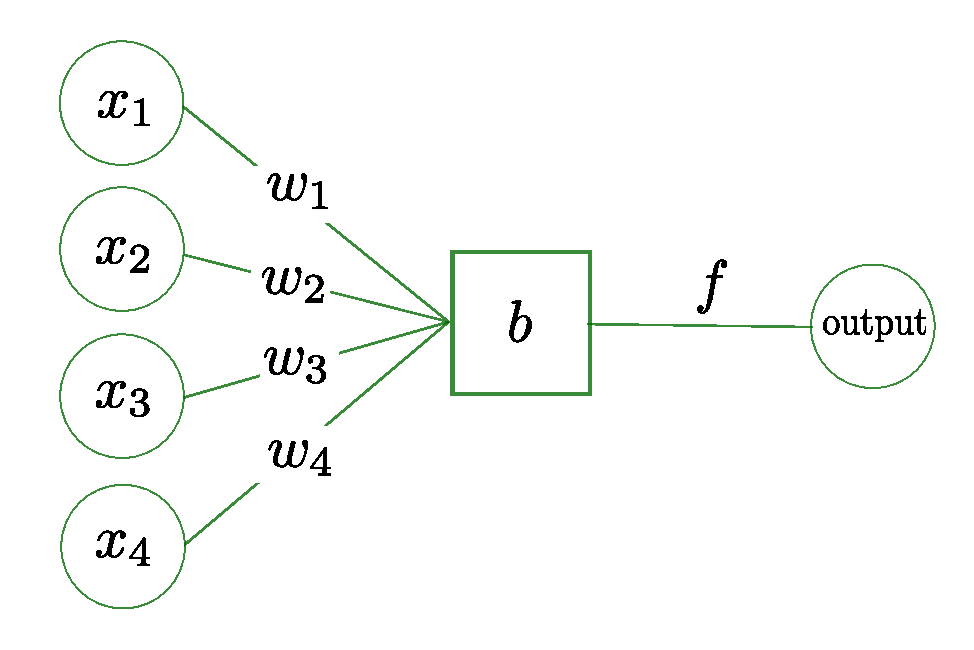
\includegraphics[width=0.6\columnwidth]{C4_cnn/neuron.pdf}
    \caption{Basic neuron}
    \label{machine:nn:neuron:plot}
\end{figure}

In the example in Fig.~\ref{machine:nn:neuron:plot} I have shows a neuron which has 4 input variables, or 4 input data points. 
When a network is trained, or when it learns, the weights applied to each of the inputs and the bias are updated to better represent the input data.
This training procedure is explained in more detail in Sec.~\ref{machine:nn:training}
Many neurons are then used in combination with each other to develop a neural network which can be applied to more complex problems.

%%%%%%%%%%%%%%%%%%%%
\subsection{\label{machine:nn:structure}Network structure}
%%%%%%%%%%%%%%%%%%%%

The structure of a neural network is defined by the user and there is no set way to design a network.
However, the general layout of a neural network is defined by structures called layers, sometimes known as fully connected layers. 
These are rows of $N$ neurons which all take the same input such that there is $N$ output values.
An example of a simple neural network is shown in Fig.~\ref{machine:nn:structure:plot}.
The first layer is the input layer, this is just the data points from an input example.
In the example of hand drawn digits, this would be the pixels from the image of the digit.
The final layer represents the information that you intend the network to extract from the input data. 
In the hand drawn digit example, this could have 10 output values corresponding to each digit 0-9. 
Each of these outputs is then a value which is related to the probability of that digit being present in the image.  

When designing a network, the user will have a defined input layer size from the data and a set number for the output layer which represents, for a classification example, the number of output classes. 
The number of hidden layers and the number of neurons in those hidden layers can be arbitrarily changed. 
In general if the data contains more complex information the size or complexity of the network will need to be increased for it to be able to extract the information. 
If there is a small number of training examples and a large and complex network, it may be able to learn the input data set as opposed the the general information that they represent.

\begin{figure}[h]
    \centering
    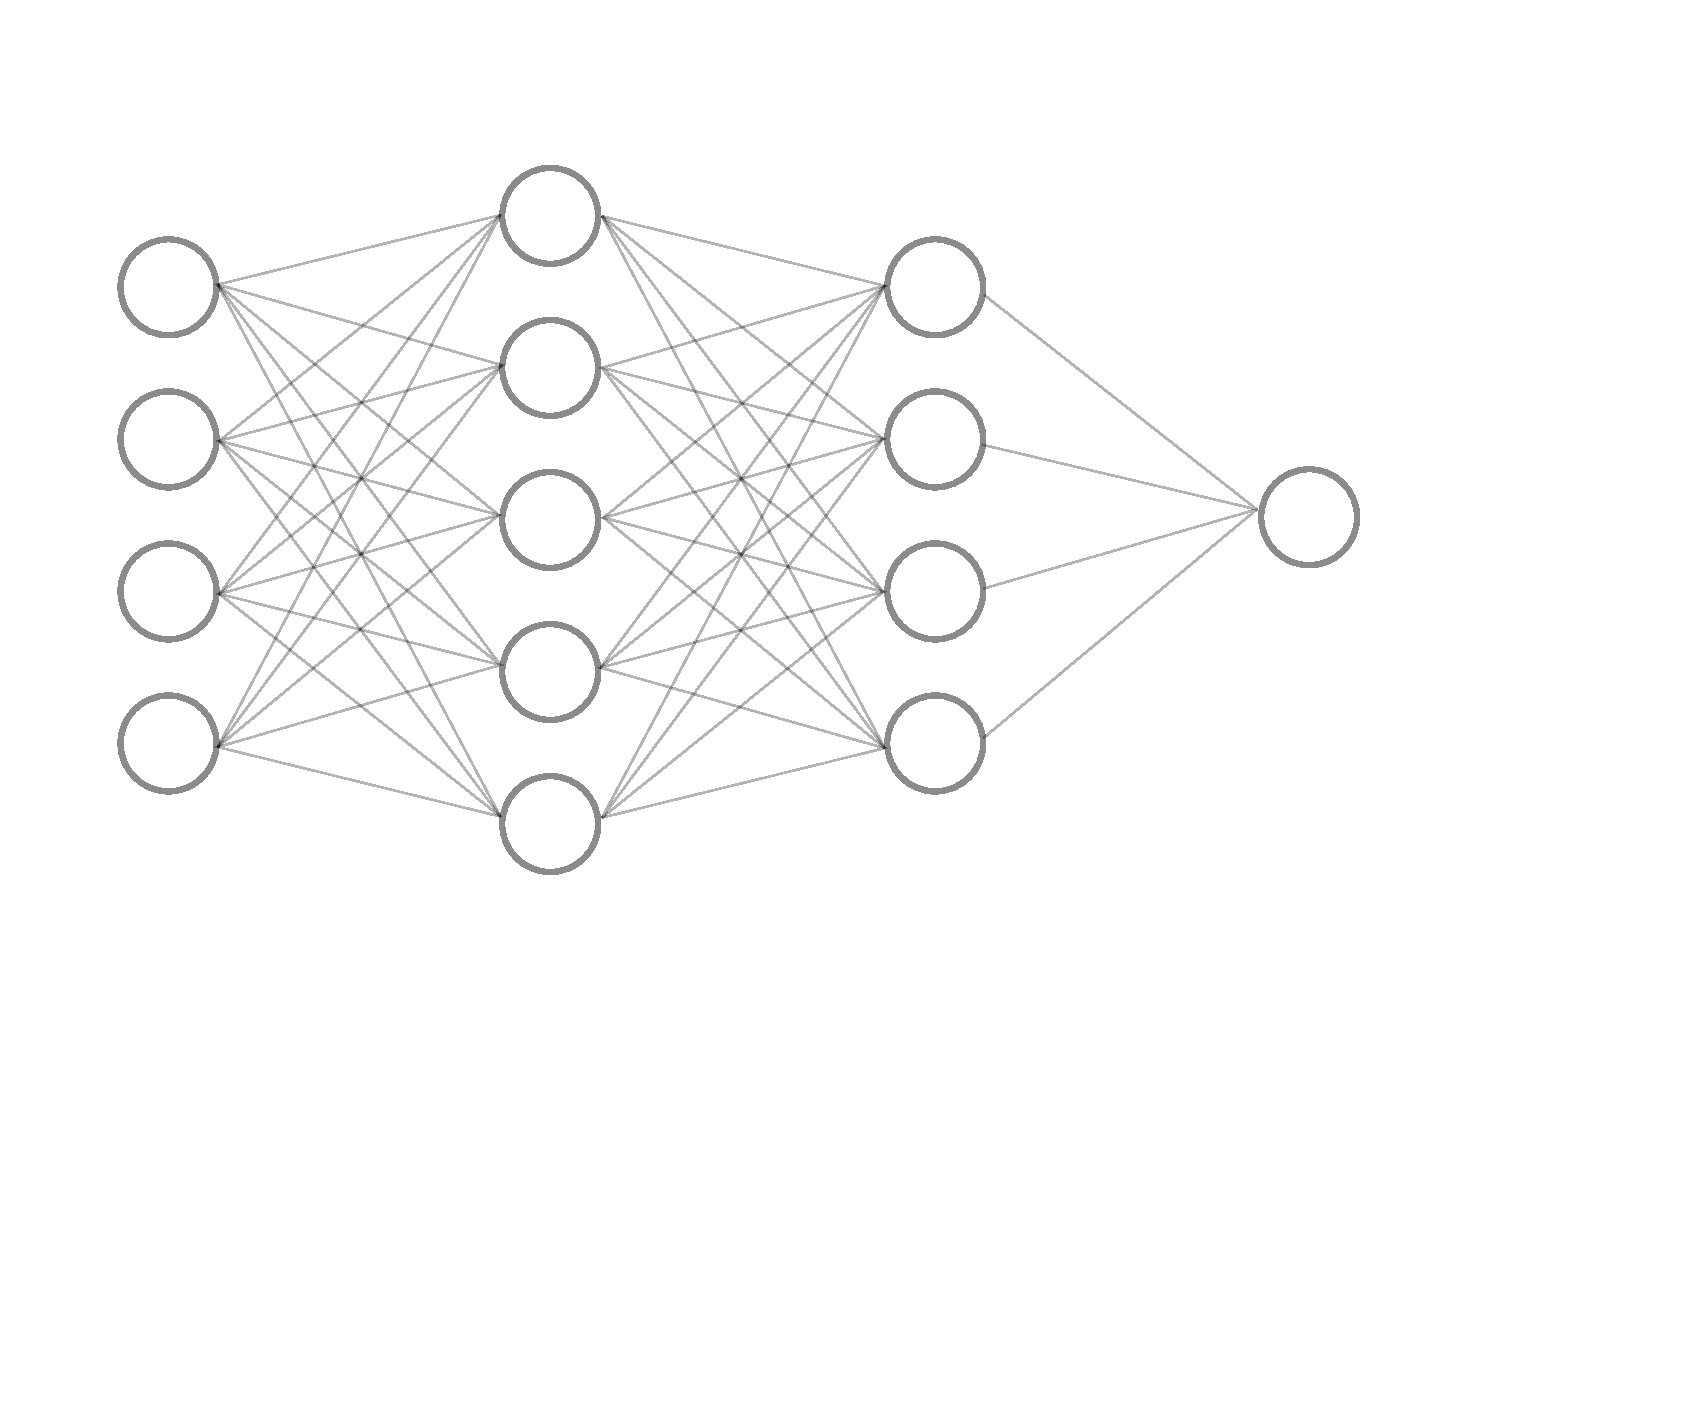
\includegraphics[width=\columnwidth]{C4_cnn/simple_network.pdf}
    \caption{A neural network is structured with layers. This consists of the input layer which is the data which you would like to analyse. Then this passes to a number of `hidden' layers, in the above diagram there are two. These are just all layers between the input and the output. The output layer is then the desired output, above there is a single neuron as output, so this could perhaps classify the input to a value between 0 and 1. Every neuron in a layer is connected to the output of all neurons in the previous layer.}
    \label{machine:nn:structure:plot}
\end{figure}


%%%%%%%%%%%%%%%%%
\subsection{\label{machine:nn:activation}Activation functions}
%%%%%%%%%%%%%%%%%

The activation function is how the output of a neuron is transformed. 
The most simple activation function is a cut as described in Sec.~\ref{machine:nn:neuron}, however, this type of activation does not perform well.
Activations functions a generally based on a few properties.
The activation function is generally non-linear, this allows networks with multiple layers to be used to approximate a function. A linear activation function means that any number of layers in a network is equivalent to a single layer network.
Another property which is desired in activation function is that it is continuously differentiable. This is to allow algorithms such as gradient descent to optimise the network. 
The functions are found to perform better if they are monotonic and smooth.
There are many choices when defining this in the network, some of the available options are shown in Fig.~\ref{machine:nn:activation:plot}.
One of the more commonly used activation function is the LeakyRELU function, this is explained in more detail in \citep{maas2013RectifierNonlinearities}.
In the work that follows we use the Leaky RELU function and the sigmoid function.


\begin{figure}[h]
	\centering
	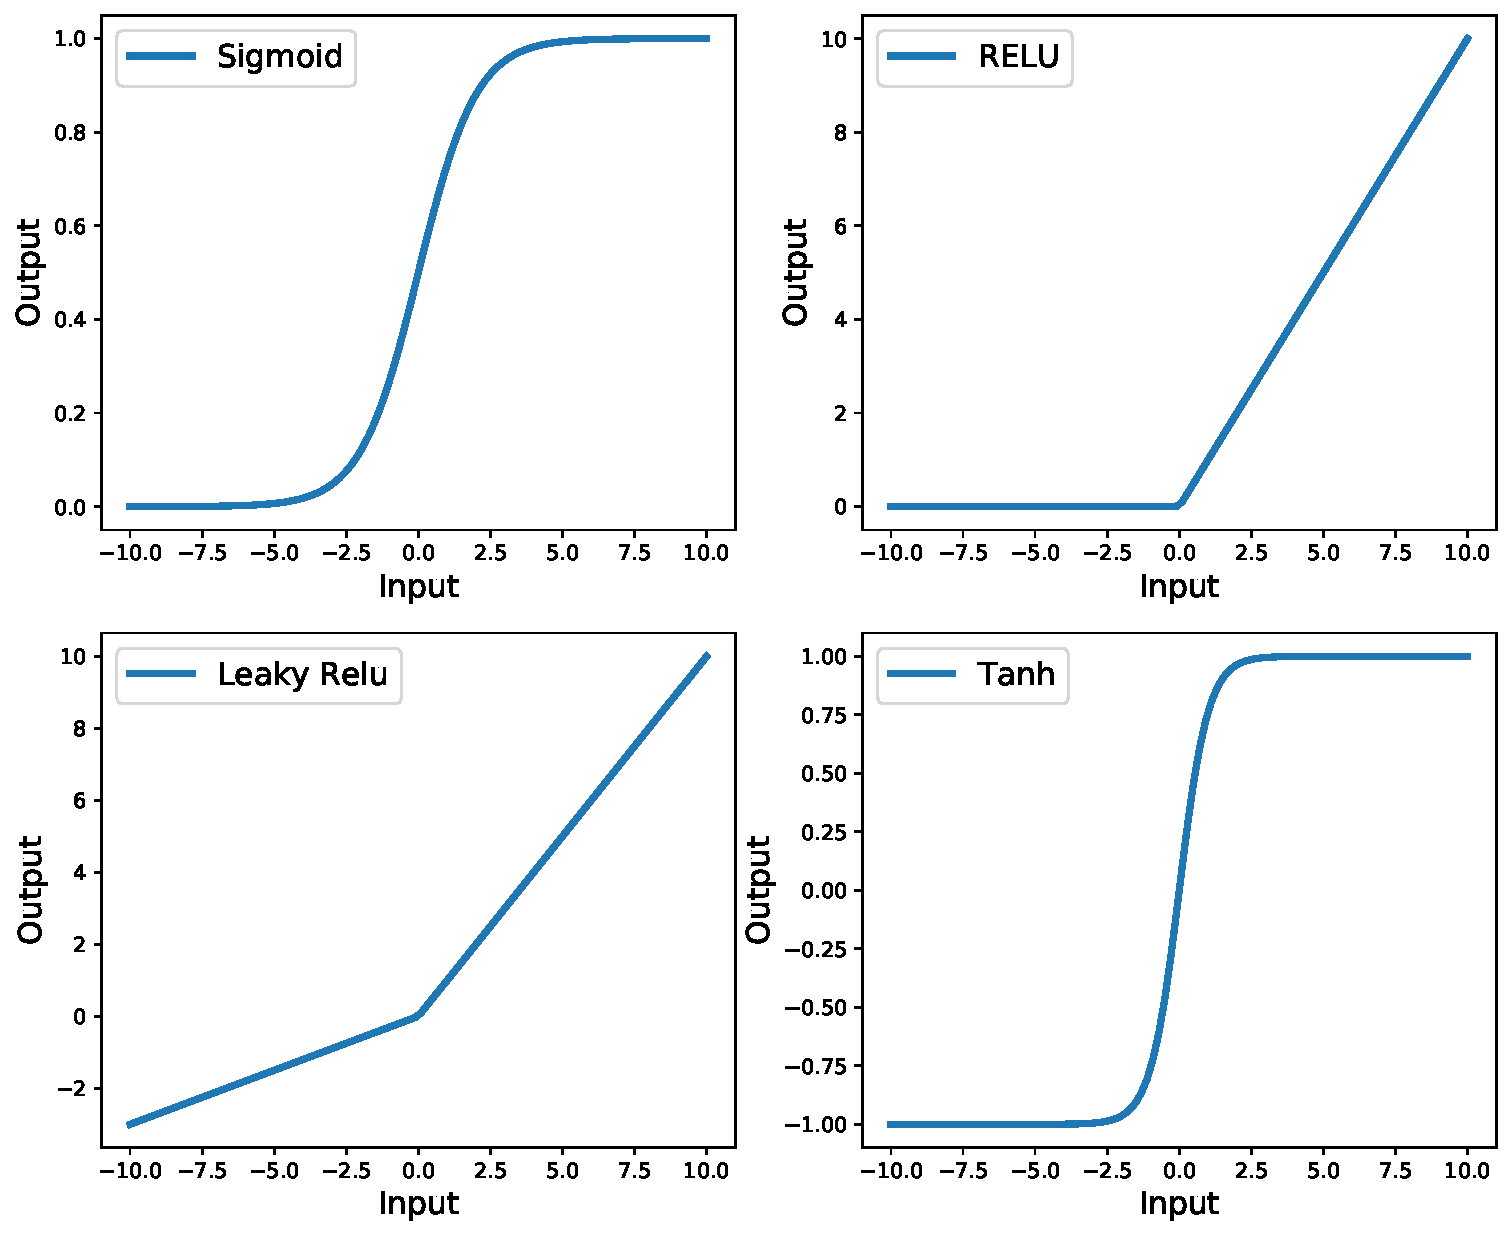
\includegraphics[width=\columnwidth]{C4_cnn/activations.pdf}
	\caption{There are many different activations function which are used, and essentially any function can be defined if necessary. Above is shown a subset of the more commonly used functions. The linear function is not used, however, is there to compare to common non linear function.}
	\label{machine:nn:activation:plot}
\end{figure}


%%%%%%%%%%%%%%%%%
\subsection{\label{machine:nn:training}Training}
%%%%%%%%%%%%%%%%%

% introduce training concept
%
Once the structure of the network is decided, the network needs to be trained.
This means that the weights and bias' for every neuron need to be updated such
that the neural network gives a useful output. For this
work we will classify the input images using a single output neuron.
This neuron outputs a value between 0 and 1 using a sigmoid function.
The \ac{CNN} is trained using a process called supervised
learning. When using supervised learning, the class of each input example is know. For example, we assign a label of 1 when the
input is a time-frequency spectrogram which includes a simulated \ac{CW}
signal. Similarly a time-frequency spectrogram with no simulated signal is assigned a label of 0. 
In general when training neural networks this way, the performance of the network can be improved by increasing the number of input examples which are shown to the network.
This stops the network from over-fitting to specific examples. Instead it should generalise to the full input and learn the underlying features within the data.

%Training procedure
%
Each of the training examples is then propagated though the network to its single output value which lies between 0 and 1. Using a loss function, this output is then be compared to
the label of the input data which is either 0 or 1. As we are classifying
between two classes in out networks, the loss function, $L$, is the binary
crossentropy defined as,
%
\begin{equation}\label{cnn:loss} 
L = -y\log{(p)} + (1-y)\log{(1-p)},
\end{equation}
%
where $p$ is the networks predicted output which has any value in the range $[0,1]$ and $y$ is the true output which has binary labels 0 or 1. 
The loss function is minimised when the output matches the truth. This essentially
tells the neural network how close to the truth it is. The weights and bias' of
the neural network can be updated based on the value of this loss function. The
process of updating the weights and other parameters is called back-propagation,
and typically uses a form of gradient descent
\cite{kingma2015AdamMethod}.
Back-propagation uses the derivative of the loss function with respect to a weight to update that weight.
If changing that weight in a particular direction decreases the loss function, then the weight will be updated in that direction.
The size of the change of the weight value is related to the change in the size loss function.
This means that the weights can be updated to minimise the loss function and therefore improve the performance of the network.



%%%%%%%%%%%
%%%%%%%%%%%
\section{Convolutional Neural Networks}
%%%%%%%%%%%
%%%%%%%%%%%

Convolutional neural networks are based on the same principles as the neural networks described above. 
The difference being that \acp{CNN} use additional types of layers which help to retain information of pixels relative to each other.
In a standard neural network, it does not have any information on the location of any input value.
For example, in an input image every pixel is flattened into a single dimensional array before being input to the network.
\acp{CNN} try to retain some location information for each of the pixels.
Whilst \acp{CNN} can be used for single dimensional inputs, they were generally developed for images.
As well as retaining some location information, they reduce the size of the networks parameters.


%%%%%%%%%%
%%%%%%%%%%
\subsection{Convolutional layers}
%%%%%%%%%%
%%%%%%%%%%

Convolutional layers have some similarities to standard fully connected layers as described in Sec.~\ref{machine:nn:structure}. 
The main difference being how the weights are applied to the inputs.
To show the difference I have an example of a simple input image which has 9 pixels, this is shows in Fig.~\ref{}.

A fully connected neural network would flatten this image and apply Eq.~\ref{machine:nn:neuron:equation} to the inputs, such that the output is,

\begin{equation}
\begin{split}
    O_{k} &= f\left(\sum_{i} \sum_{j} I_{i,j} w_{i,j,k} + b_k \right) \\
    O_1 &= f\left(I_1 w_{1,1} + I_2 w_{2,1} + I_3 w_{3,1} + I_4 w_{4,1} + I_5 w_{5,1} + I_6 w_{6,1} + I_7 w_{7,1} + I_8 w_{8,1} + I_9 w_{9,1} + b_1\right) \\
     \dots
\end{split}
\end{equation}

If the size of the convolutional filter was $2\times 2$, then the convolutional layer only has 5 parameters to vary as opposed to 10 in this case.
This would then use the equation,
\begin{equation}
    O_{i,j} = \sum_{m} \sum_{n} K_{m,n}I_{i-m,j-n}
\end{equation}
\begin{equation}
\begin{split}
    O_1 &= f\left(I_1 w_1 + I_2 w_2 + I_4 w_3 + I_5 w_4 + b\right) \\
    O_2 &=  f\left( I_2 w_1 + I_3 w_2 + I_5 w_3 + I_5 w_4 + b\right)\\
    O_3 &=  f\left(I_4 w_1 + I_5 w_2 + I_7 w_3 + I_8 w_4 + b\right)\\
    O_4 &=  f\left(I_5 w_1 + I_6 w_2 + I_8 w_3 + I_9 w_4 + b\right).
\end{split}
\end{equation}

Whilst this is hard to picture mathematically, it can be easier seen as a 2x2 filter which is convolved with the input image. 
Fig.~\ref{} shows how the convolutional filter is applied.
The output of a convolutional layer is then an image which is half the filter length less length in each dimension. 
In practice, the input images are often padded with zeros such that the output image is the same size as the input image. 

\begin{figure}[h]
\begin{subfigure}[h]{\columnwidth}
    \centering
    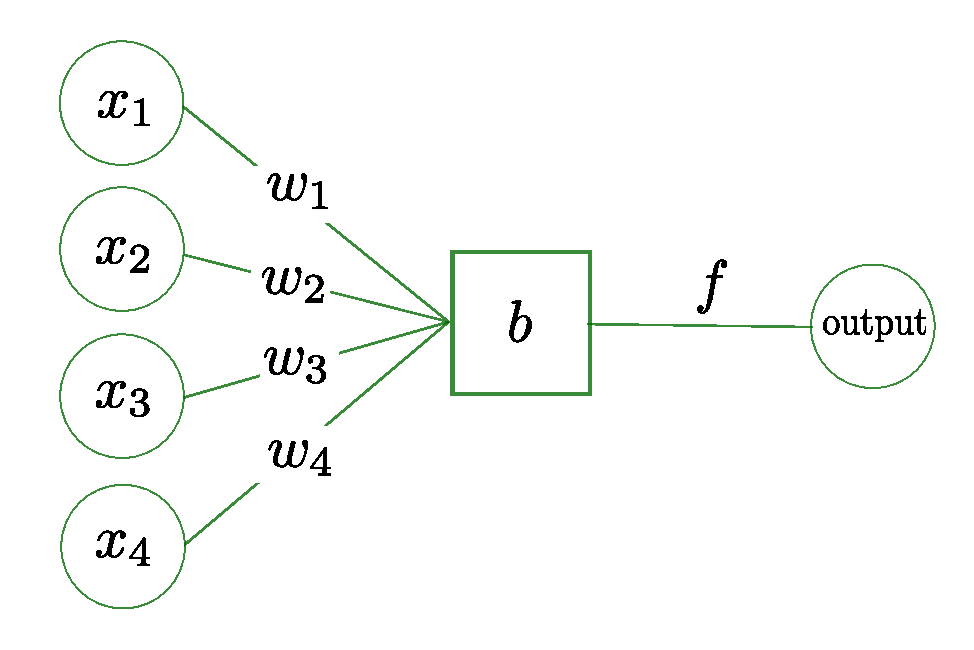
\includegraphics[width=0.5\columnwidth]{C4_cnn/neuron.pdf}
    \caption{Simple neural network}
    \label{machine:cnn:convlayer:input}
\end{subfigure}   

\begin{subfigure}[h]{\columnwidth}
    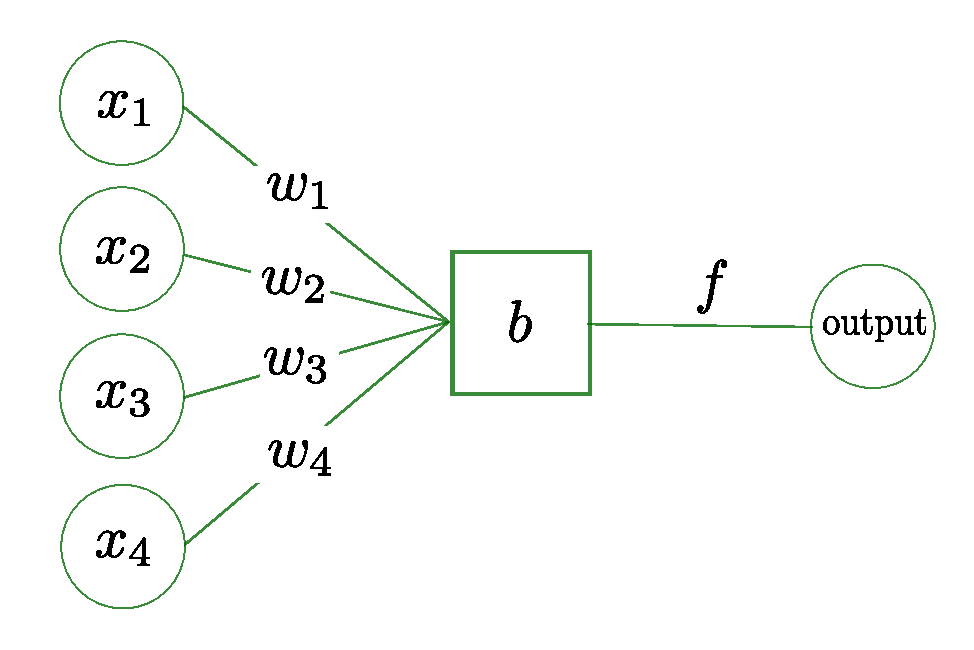
\includegraphics[width=0.5\columnwidth]{C4_cnn/neuron.pdf}
    \caption{Simple neural network}
    \label{machine:cnn:convlayer:nn}
\end{subfigure} 

\begin{subfigure}[h]{\columnwidth}
    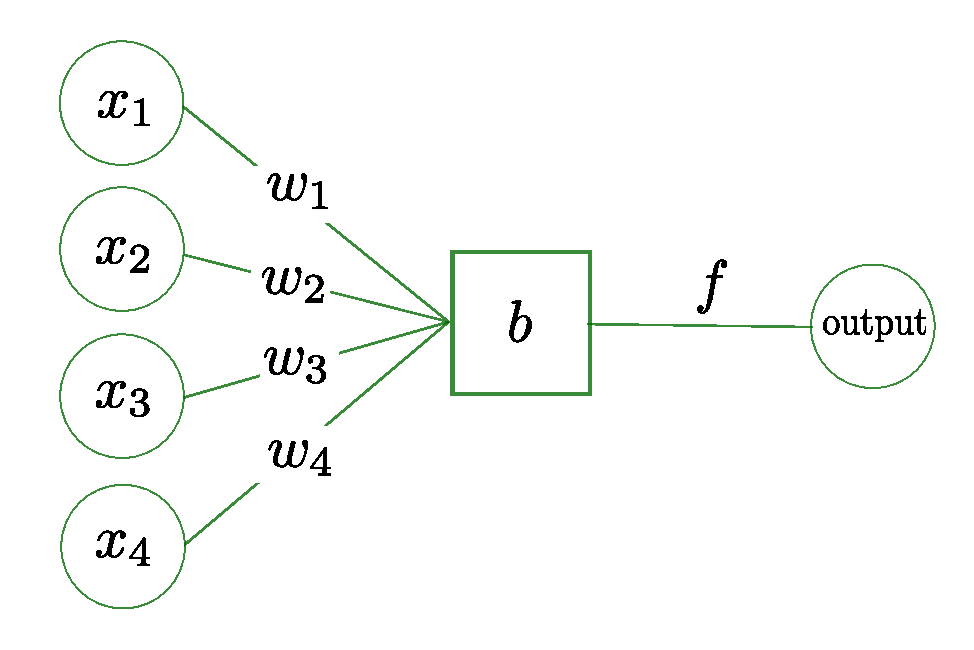
\includegraphics[width=0.5\columnwidth]{C4_cnn/neuron.pdf}
    \caption{Simple neural network}
    \label{machine:nn:convlayer:cnn}
\end{subfigure} 

\end{figure}

A convolutional layer has a number of different parameters which can be varied when setting up a model.
Below I list each of the adaptable parameters and what they do.

\begin{description}
\item[Filter size] The filter size is the size and shape of the convolutional filter. The filter does not have to be square, however must be less than the dimensions of the image.

\item[Number of filters] The number of filters can be any value. If you have $K$ filter kernels, then the convolutional layer will output $K$ filtered images.

\item[Activation function] The activation function is generally kept the same for each of the layers, however this can be set here. The different types have been explaine in Sec.~\ref{machine:nn:activation}.

\item[Stride] The stride is when the convolution is applied to every other pixel. This method reduces the size of the output by the same factor. This is not used in the rest of this work.
\end{description}

The convolutional layers with reduce the number of parameters used in each network or model, which can speed up the training procedure.
In a normal neural network the image is flattened, therefore, any information which related the location of a pixel to another is lost. 
Convolutions can keep hold of this information and look for similar patters within an image.

%%%%%%%%%
%%%%%%%%
\subsection{Max pooling layers}
%%%%%%%%%%%%
%%%%%%%%%%%

Max pooling layers are designed to reduce the size of the problem whilst holding on to as much important information as possible.
the idea of this layer is relatively simple, it reduces the image size by taking the maximum value in a reigon of a given size.
For example, in Fig.~\ref{maxpool}, the image is reduced by a 2x2 max pooling layer.

\begin{figure}
    \centering
    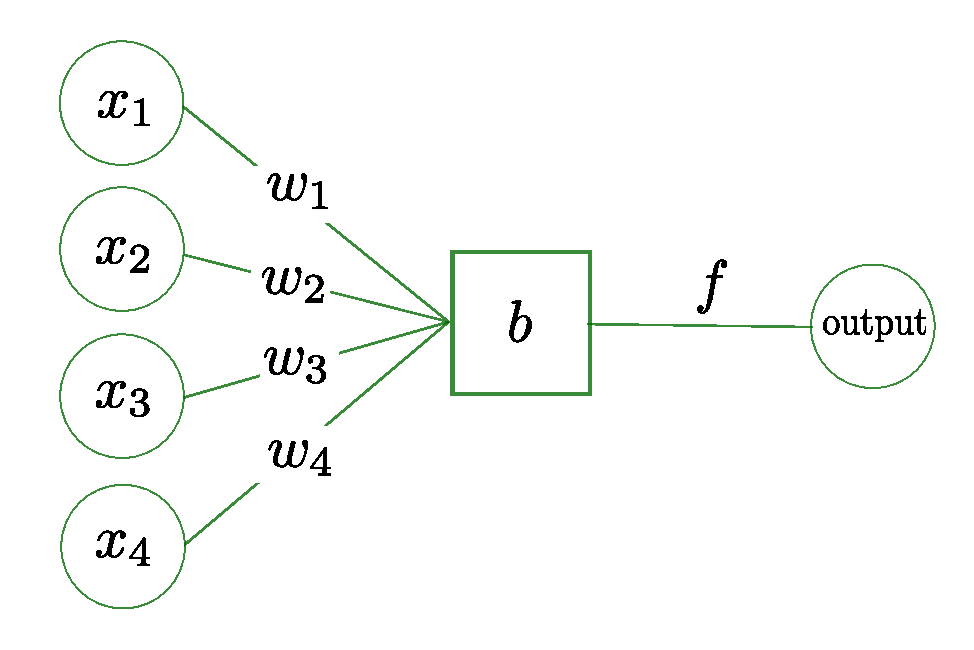
\includegraphics[width=0.5\columnwidth]{C4_cnn/neuron.pdf}
    \caption{Max pooling layer}
    \label{fig:my_label}
\end{figure}

%%%%%%%%%%%%%
%%%%%%%%%%%%%%
\subsection{CNN structure}
%%%%%%%%%%%%%%
%%%%%%%%%%%%%%

\acp{CNN} are usually structured such that they can extract larger features from an input image, then the outputs from this are passed on to be classified.
To extract the larger features any number of different convolutional layers and max-pooling layers used.
Once this then outputs $K$ images, the values are flattened into a one dimensional array an passed to a set of fully connected layers. 
This is essentially the same type of network described in Sec.~\ref{machine:nn}.
This can then classify the network into the chosen output.

\acp{CNN} are then trained in the same way as neural networks as described in Sec.~\ref{machine:nn:training}.

%%%%%%%%%%%%%%%%%%%%%%%%%%%%%%%%%%%%%%%%%%%%%%
%%%%%%%%%%%%%%%%%%%%%%%%%%%%%%%%%%%%%%%%%%%%%%%%
\section{CW search}
%%%%%%%%%%%%%%%%%%%%%%%%%%%%%%%%%%%%%%%%%%%%%%%%%
%%%%%%%%%%%%%%%%%%%%%%%%%%%%%%%%%%%%%%%%%%%%%%%




%%%%%%%%%%%%%%%
%%%%%%%%%%%%5%%
\subsection{Network structure}
%%%%%%%%%%%%%%%
%%%%%%%%%%%%%%%

\subsubsection{Viterbi statistic}

\subsubsection{Viterbi Maps}

\subsubsection{Spectrograms}

\subsubsection{Viterbi map and spectrograms}

\subsubsection{Viterbi map and Viterbi statistic}

\subsubsection{Viterbi map, Viterbi statistic and spectrograms}

%%%%%%%%%%%
%%%%%%%%%%%
\section{\label{cnn:networkvis}Network Visualisation}
%%%%%%%%%%%
%%%%%%%%%%%

Neural network are generally hard to visualise due to the large number or parameters in the network that have to be varied.
However, there are methods which can be used to see how input data is affected by the network.
This can be useful to see how the network performs when given certain types of data and gives some insight into how the networks work

In the examples above we use \acp{CNN}, the first few layers of this are build using convolutional filters.
The filters weights should ideally correspond to the shape of the feature which one wants to extract from the image. 
Generally this is only useful to picture at the first layer as the network can make subsequent layer and representations quite abstract.



\begin{figure}[h]
	\centering
	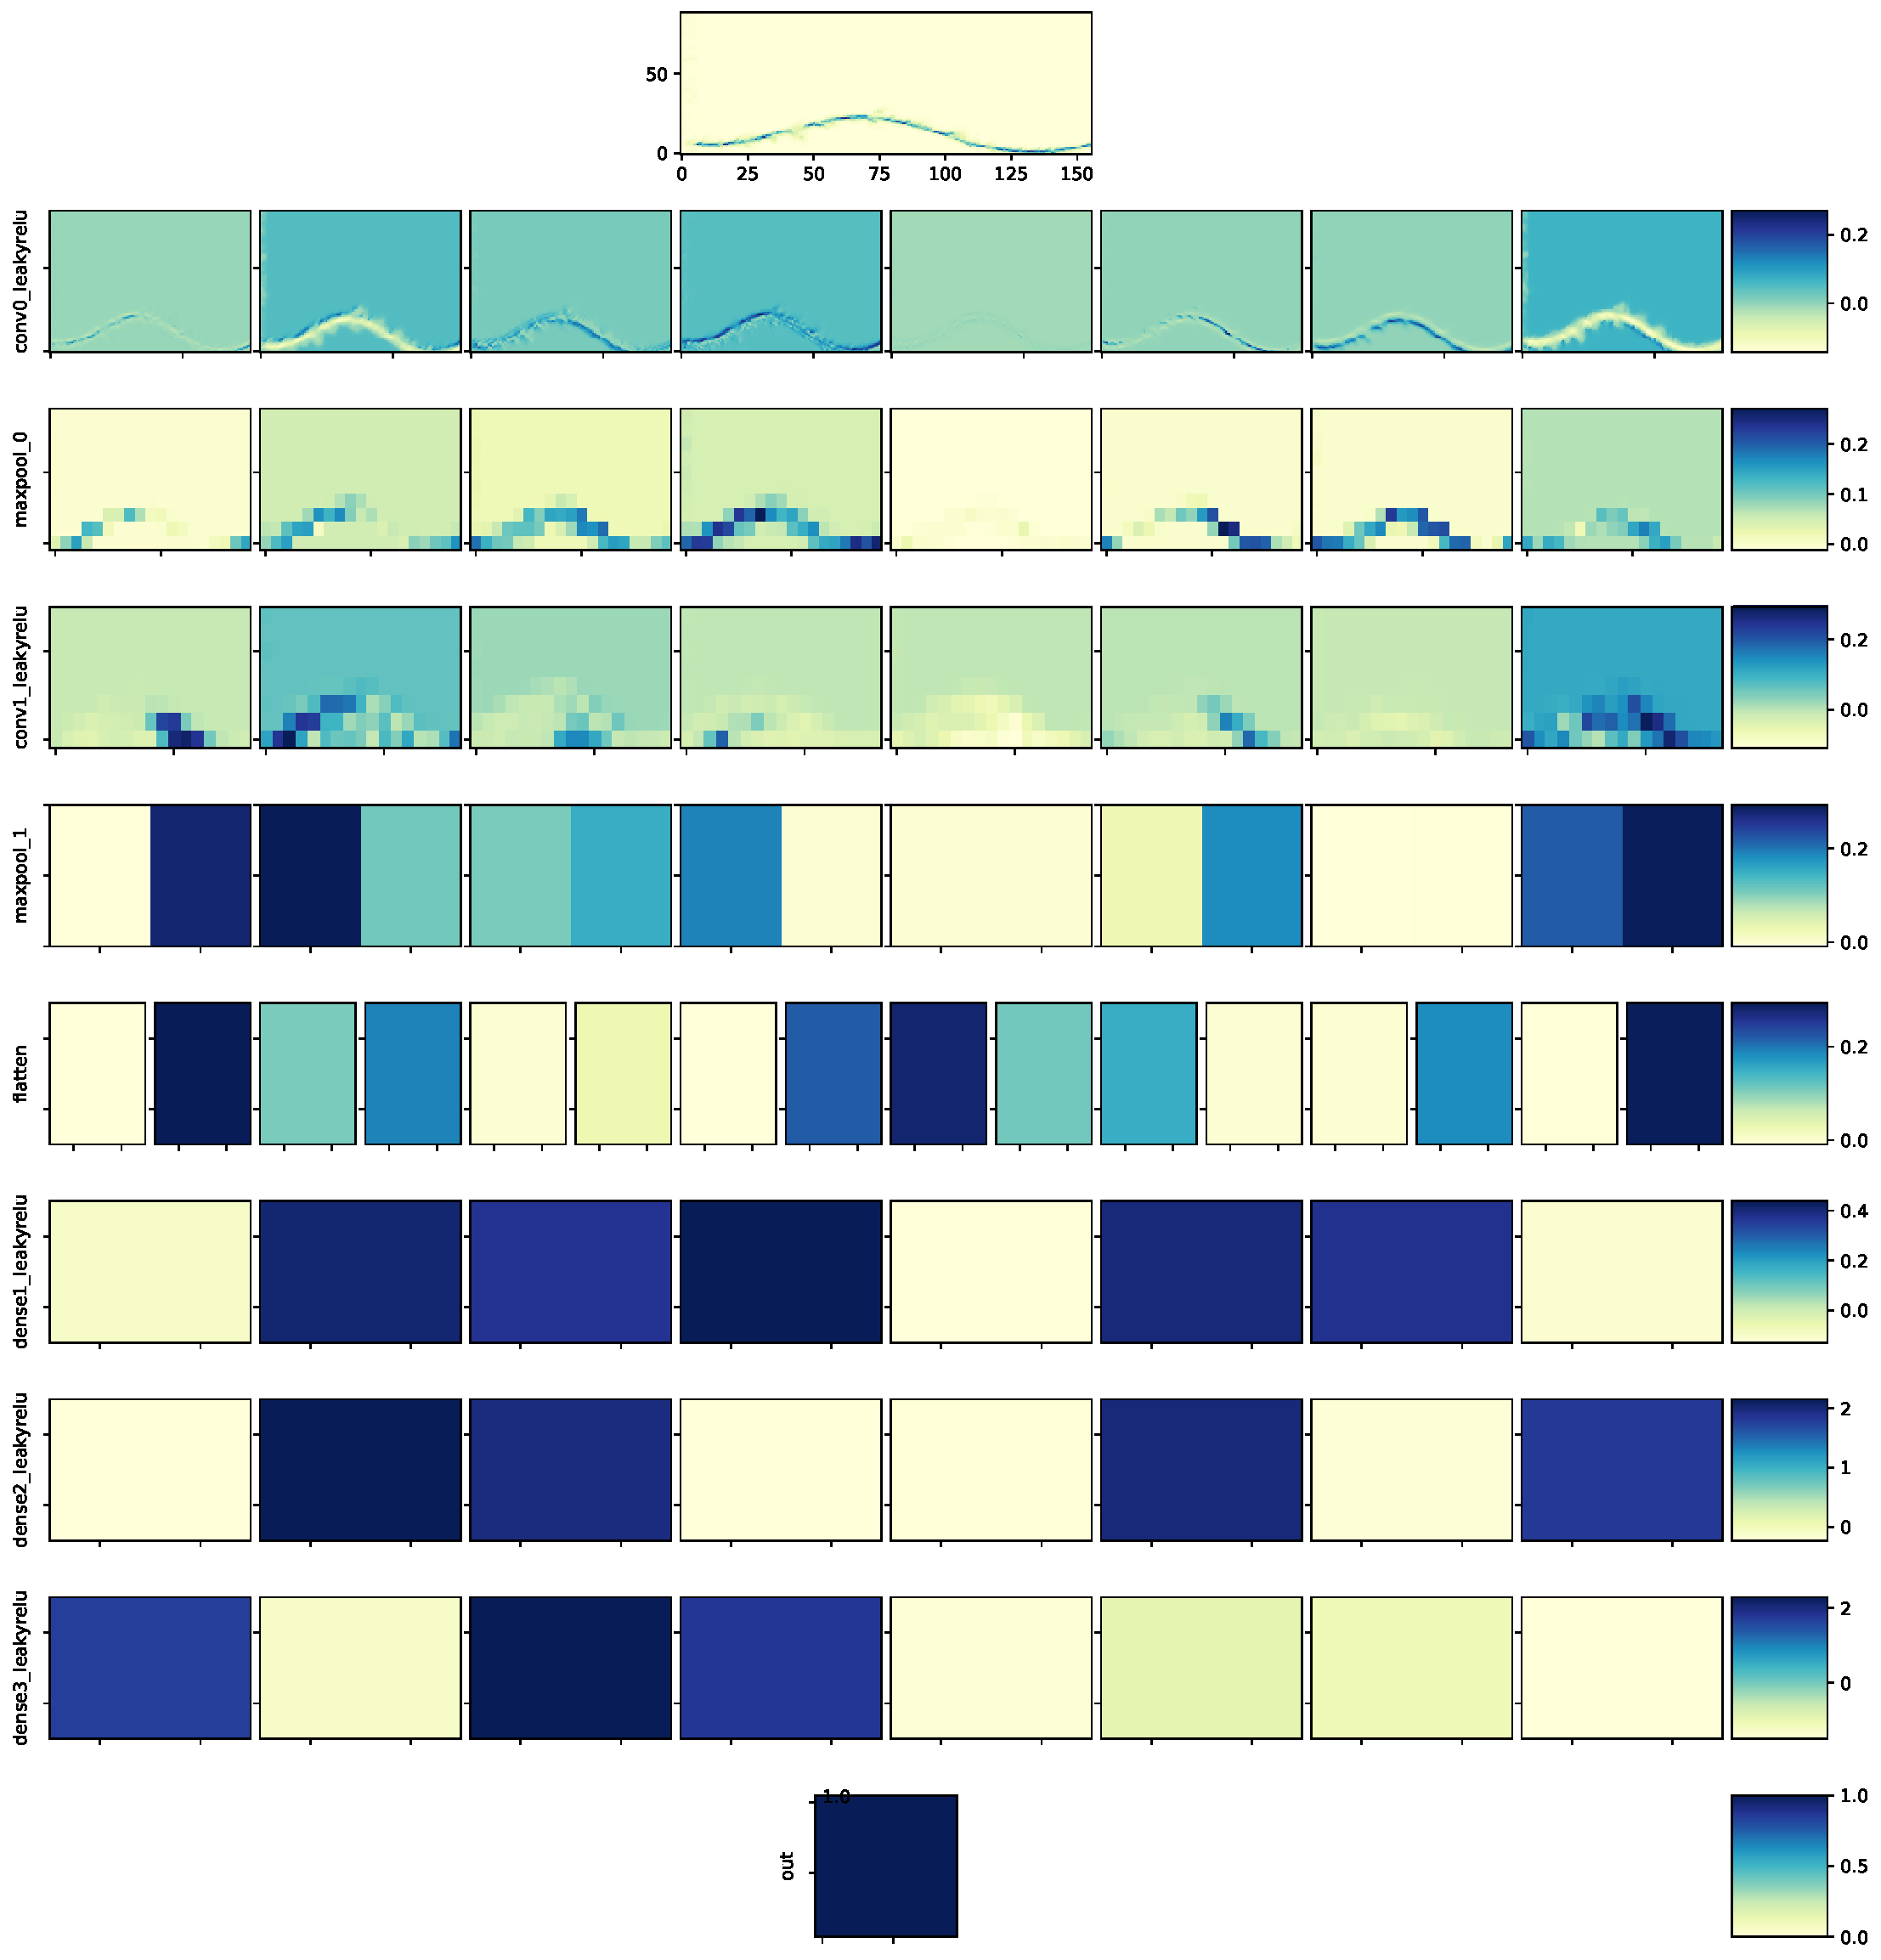
\includegraphics[width=\textwidth]{C4_cnn/vitmap_cnn_visualisation_signal.pdf}
	\caption{This shows a visualisation of the convolution neural network used for vitebri maps above}
	\label{cnn:vis:vitmap:signal}
\end{figure}


%%%%%%%%%
%%%%%%%%%%%
\section{Data and simulations}
%%%%%%%%%%
%%%%%%%%%%%